\documentclass[a4paper,11pt,twoside,fleqn,openright]{memoir}
 
% Pakker
\usepackage[utf8]{inputenc} % Så må vi bruge æ, ø og å
%\usepackage[ansinew]{inputenc}
%\usepackage[danish]{babel} % Dansk opsætning
\usepackage[T1]{fontenc} % Hjælper med ordeling ved æ, ø og å. Sætter fontene til at være ps-fonte i stedet for bmp.
%\usepackage[scaled]{beramono} % Bedre monospace font
\usepackage{amsmath,amsfonts,amssymb} % God matematik
\usepackage{sistyle} % Enheder til fysik
\usepackage{array,booktabs} % Til gode tabeller
\usepackage{ragged2e} % For at kunnu lave tabeller med fast kolonnebredde, bruges sammen med 'array'
\usepackage{float} % Vi må nu bruge H som placering til floats
\usepackage{hhline} % Sum linie i tabel
\usepackage{multirow} % Fletning af rækker
\usepackage{multicol} % Fletning af kolonner
\usepackage{xcolor} % Vi kan bruge \color osv
\usepackage{colortbl} % Muligøre farver i tabeller
%\usepackage[danish=quotes]{csquotes} % Danske anførselstegn, brug enquote{}
\usepackage[english=british]{csquotes} 
\usepackage{graphicx} % Inkludere ekstern grafik
\usepackage[english,final]{varioref} % Vi kan anvende \vref
\usepackage{natbib} % Bedre litteratur henvisninger
\usepackage{pdfpages} % Inkludere en pdf side som en side  
\usepackage{acronym} % Smart akronymhåndtering
\usepackage{suffix} % Krævet af acronym
\usepackage{listings} % Til at inkludere kildekode direkte
\usepackage{lipsum} % Lorem ipsum dolar sit amet
\usepackage{caption} % Vi kan bruge \captionof
\usepackage{subfig} % Vi kan nu bruge \subfloat
\usepackage{calc} % Vi kan regne med tællere
\usepackage{changepage} % Vi kan ændre sidelayoutet lokalt
\usepackage{layout} % Vi kan se dimensionecne på vores layout med \layout
\usepackage[footnote,final,english,silent,nomargin]{fixme}
\usepackage[colorinlistoftodos]{todonotes}
\usepackage[pdftex,bookmarks=true,bookmarksnumbered=true]{hyperref} % Links i dokumentet
\usepackage{textcomp} % HVAD FANDEN GØR DENNE PAKKE?
\usepackage{threeparttable} % Så vi kan lave tablenotes (se latexbogen)
\usepackage{fixltx2e} % HVAD FANDEN GØR DENNE PAKKE?
\usepackage{minitoc} % Vi kan lave del inholdsfortegnelser forhåbentlig
\usepackage{enumitem} % Better lists
\usepackage{geometry}

% For sjov pakker
\usepackage{marvosym}
\usepackage{wasysym}
%\usepackage{fourier}

\captionsetup{font={small,sf},labelfont=bf}

\pagestyle{companion}

% Andre egensakber for komandoer
\newcommand\Cpp{C\raisebox{\height / 2}[\height][\depth]{\tiny ++}} % Pænere C++
\newcommand{\mimg}[4]{\marginpar{\small \centering{\includegraphics[width=#1]{#2}\captionof{figure}{\newline #3}\label{#4}}}} % Margin billede
\newcommand{\lmimg}[4]{\marginpar{\small\centering{% Latex margin billede
  \def\svgwidth{#1}
  \graphicspath{{illustrations/}}
  \input{illustrations/#2.pdf_tex}
  \captionof{figure}{\newline #3}
  \label{#4}}}
}
\newcommand{\mnote}[1]{\marginpar{\small \textsf{\textbf{Note}\\{#1}}}} % Margin note
\newcommand{\mcd}[1]{\marginpar{\textsf{\textbf{
\includegraphics[height=11pt]{frontmatter/media-optical}}\\\url{#1}}}} % CD-rom henvisning i margin
\newcommand{\cd}[1]{
\includegraphics[height=9pt]{frontmatter/media-optical}\url{#1}} % CD-rom henvisning i tekst
\newcommand{\limg}[5]{\begin{figure}[#1]
  \centering
  \def\svgwidth{#2}
  \graphicspath{{illustrations/}}
  \input{illustrations/#3.pdf_tex}
  \caption{#4}
	\label{#5}
\end{figure}}
\newcommand{\head}[1]{{\slshape{#1}}\vspace{5mm}} % Header
\newcommand{\tail}{\vspace{3mm}\fancybreak{$*\quad*\quad*$}\vspace{3mm}} % Røvhul
\newcommand{\enhed}[1]{\hfill\hbox{[#1]}\qquad} % At indsatte heb enheder i firkantparentes i "equation"
\newcommand{\dB}[0]{\hbox{dB}} % At skrive dB oprejst
%\addto\captionsdanish{
%\renewcommand\appendixname{Appendiks}
%\renewcommand\contentsname{Indholdsfortegnelse}

% Make vectors bold instead of a arrow
\let\oldhat\hat
\renewcommand{\vec}[1]{\mathbf{#1}}
\renewcommand{\hat}[1]{\oldhat{\mathbf{#1}}}

\makechapterstyle{box}{
  \renewcommand*{\printchaptername}{}
  \renewcommand*{\chapnumfont}{\normalfont\sffamily\huge\bfseries}
  \renewcommand*{\printchapternum}{
    \flushleft
    \begin{tikzpicture}[line width=4pt]
      \draw (0,1) -- (0,0) -- (1,0);
      \draw (2,1) -- (2,2) -- (1,2);
      \draw[color=gray] (1cm,1cm) node { \chapnumfont\thechapter };
    \end{tikzpicture}
  }
  \renewcommand*{\chaptitlefont}{\normalfont\sffamily\Huge\bfseries}
  \renewcommand*{\printchaptertitle}[1]{\flushleft\chaptitlefont##1}
  \setlength\beforechapskip{-100pt}
}

\newif\ifchapternonum
\makechapterstyle{nickoe}{
\renewcommand\printchapternonum{\chapternonumtrue}
  \renewcommand*{\printchaptername}{} % Removes the 'Chapter' text
  \renewcommand*{\chapnumfont}{\fontfamily{pbk}\fontseries{m} \fontshape{n}\fontsize{80}{35}\selectfont } % Does some magic
  \renewcommand*{\printchapternum}{}
  %\hfill 
  %\fontfamily{pbk}\fontseries{m} \fontshape{n}\fontsize{80}{35}\selectfont % Makes a gigantic number
  %\chapnumfont\thechapter} % Removes the 'Chapter's number
  \renewcommand*{\printchaptertitle}[1]{%
  \noindent%
  \ifchapternonum%
  \begin{tabularx}{\textwidth}{X}%
  {\parbox[b]{\linewidth}{\raggedright \hskip -0.6em \chaptitlefont ##1}%
    \vphantom{\raisebox{0pt}{\chapnumfont 1}}}
  \end{tabularx}%
  \else

  \begin{tabularx}{\textwidth}{Xl}
  {\parbox[b]{\linewidth}{\raggedright \hskip -0.6em \chaptitlefont ##1} }
  & \raisebox{0pt}{\raggedleft \chapnumfont \hskip -0.5cm \thechapter \hskip -0.5cm}%
  \end{tabularx}%
  \fi
  \hrule
  }

  %\flushleft\chaptitlefont##1} % Prints the chaptertitle
  %\renewcommand{\afterchaptertitle}{\par\nobreak\medskip\hrule\vskip\afterchapskip}
  \setlength\beforechapskip{-100pt} % Makes the chapter go up on the page

}

\newenvironment{ffk}[0]% formel forklaring
{\begin{list}{}%
         {\setlength{\leftmargin}{\mathindent}}%
         \item[]%
}
{\end{list}}

% Akronyms formatering
\renewcommand*{\acsfont}[1]{#1}
\renewcommand*{\acffont}[1]{#1}
\renewcommand*{\acfsfont}[1]{#1}

% Farve definitioner
\definecolor{shadecolor}{gray}{.95}

\lstloadlanguages{C,VHDL,Java}
% Kodeformatering [C]
\lstnewenvironment{ccode}[2][]{
  \def\lstlistingname{Source code}
  \lstset{
    language=C,
    escapeinside={(*@}{@*)},  % a line can set with: (*@\label{c:labelname}@*)
    keywordstyle=\bfseries,
    commentstyle=\color{blue}, 
    basicstyle=\ttfamily\selectfont\footnotesize,
    numbers=left,
    numberstyle=\tiny,
    tabsize=2,
    showstringspaces=false,
    backgroundcolor=\color{shadecolor},
    frame=lines,
    captionpos=b,
    caption={#1},
    label={#2}
  }
}{}

% Kodeformatering [VHDL]
\lstnewenvironment{VHDL}[2][]{
  \def\lstlistingname{Source code}
  \lstset{
    language=VHDL,
    keywordstyle=\bfseries,
    commentstyle=\color{blue}, 
    basicstyle=\ttfamily\selectfont\small,
    numbers=left,
    numberstyle=\tiny,
    tabsize=2,
    showstringspaces=false,
    backgroundcolor=\color{shadecolor},
    frame=lines,
    captionpos=b,
    caption={#1},
    label={#2}
  }
}{}

% Kodeformatering [Assembler]
\lstnewenvironment{asmcode}[2][]{
  \def\lstlistingname{Source code}
  \lstset{
    language=[x86masm]Assembler,
    keywordstyle=\bfseries,
    commentstyle=\color{blue}, 
    basicstyle=\ttfamily\selectfont\small,
    numbers=left,
    numberstyle=\tiny,
    tabsize=2,
    showstringspaces=false,
    breaklines=true,
    backgroundcolor=\color{shadecolor},
    frame=lines,
    captionpos=b,
    caption={#1},
    label={#2}
  }
}{}

% Kodeformatering [Java]
\lstnewenvironment{javacode}[2][]{
  \def\lstlistingname{Source code}
  \lstset{
    language=Java,
    keywordstyle=\bfseries,
    commentstyle=\color{blue}, 
    basicstyle=\ttfamily\selectfont\small,
    numbers=left,
    numberstyle=\tiny,
    tabsize=2,
    showstringspaces=false,
    breaklines=true,
    backgroundcolor=\color{shadecolor},
    frame=lines,
    captionpos=b,
    caption={#1},
    label={#2}
  }
}{}

% Kodeformatering [XML]
\lstnewenvironment{xmlcode}[2][]{
  \def\lstlistingname{Source code}
  \lstset{
    language=XML,
    keywordstyle=\bfseries,
    commentstyle=\color{blue},
    basicstyle=\ttfamily\selectfont\small,
    numbers=left,
    numberstyle=\tiny,
    showstringspaces=false,
    backgroundcolor=\color{shadecolor},
    frame=lines,
    morekeywords={msgid, repeat, mmsi, navstat, rot, sog, posaccu, lon, lat, cog, truehead, timestamp, manoeuvre, raim, commstate, utc_year, utc_month, utc_day, utc_hour, utc_min, utc_sec, txbcast, name, aisver, imo, call, cargo, a, b, c, d, fixdev, eta_mon, eta_day, eta,hour, eta_min, draught, dest, dte, spare},
    captionpos=b,
    breaklines=true,
    caption={#1},
    label={#2}
  }
}{}

% \part omdefinering, nu med beskrivende tekst
\def\descpart#1#2{
  \par\newpage\clearpage % Page break 
  \vspace*{5cm} % Vertical shift 
  \refstepcounter{part}% Next part
  %\addcontentsline{toc}{part}{\texorpdfstring{\rlap{\thepart}\hspace{1.2em}#1}{\thepart\ #1}} % Adds entry to TOC 
  \addcontentsline{toc}{part}{\texorpdfstring{\rlap{\thepart}\hspace{2em}#1}{\thepart\ #1}} % Adds entry to TOC 
  {\centering \textbf{\Huge Part \thepart}\par}
  \vspace{1cm} % Vertical shift
  \thispagestyle{chapter} % Gives the pagestile an the memoir chapterpagestyle
  {\centering \textbf{\Huge #1}\par}
  \begin{center}
  {\parbox{9cm}{
  \vspace{2cm} % Vertical shift
  \noindent \slshape{#2} % Some text
  }}
  \end{center}
  \vfill\pagebreak % Fill the end of page and page break
}

%------------
\def\appendixpart#1#2{
  \par\newpage\clearpage % Page break 
  \vspace*{5cm} % Vertical shift 
  \addcontentsline{toc}{part}{\texorpdfstring{\rlap{\thepart}\hspace{2em}#1}{\thepart\ #1}} % Adds entry to TOC 
  \thispagestyle{chapter} % Gives the pagestile an the memoir chapterpagestyle
  {\centering \textbf{\Huge #1}\par}
  \begin{center}
  {\parbox{9cm}{
  \vspace{2cm} % Vertical shift
  \noindent \slshape{#2} % Some text
  }}
  \end{center}
  \vfill\pagebreak % Fill the end of page and page break
}


%------------

% At bruge figurer der fylder mere end brødteksten
% Der defineres nogle ekstra længder
\newlength{\fullwidth}
\setlength{\fullwidth}{\textwidth}
\addtolength{\fullwidth}{\marginparsep}
\addtolength{\fullwidth}{\marginparwidth}
\newlength{\fullmargin}
\setlength{\fullmargin}{\marginparwidth}
\addtolength{\fullmargin}{\marginparsep}
% For at bruge det, skal man f.eks. gøre således:
%\begin{figure}[h]
%\begin{adjustwidth*}{-\fullmargin}{}
%\includegraphics[width=\fullwidth]{./sti}
%\end{adjustwidth*}
%\caption{Beskrivelse her}
%\laber{fig:label}
%\end{figure}

% \degC for grader C
% \arcdeg for gradtegn
\renewcommand{\epsilon}{\varepsilon}
\newcommand{\MATLAB}{M{\footnotesize ATLAB}}
\parindent 8pt

% Orddeling
% Ord der deles forkert kan skrives her, men bindestreg ved stavelser og mellemrum mellem ordene
\hyphenation{ar-bejds-in-ten-si-ve an-grebs-vink-ler ind-gangs-im-pe-dans ro-ta-ti-ons-en-ko-der deres clock-fre-kvens sys-tem-et na-vi-gate} 


\hypersetup{
  pdftitle={AAUB\AA D},
  pdfsubject={6th semester of Electronics and IT, Aalborg University},
  pdfauthor={Brian Bach Nielsen, Nick \O stergaard, Simon Als Nielsen, Rasmus Lundgaard Christensen and Christoffer Stagsted Andreassen},
  pdfcreator=LaTeX,
  linkcolor=black,
  citecolor=black,
  filecolor=black,
  urlcolor=black
}

\begin{document}

% Frontpage
% \newgeometry{left=3cm,top=3cm,right=3cm,bottom=3cm}
\author{Nick Østergaard and Jeppe Dam}
\title{\textbf{\emph{Formation Control for Unmanned Surface Vehicles for Surveying Purposes}}}
\date{\today}
\maketitle
\thispagestyle{empty}
\begin{center}
	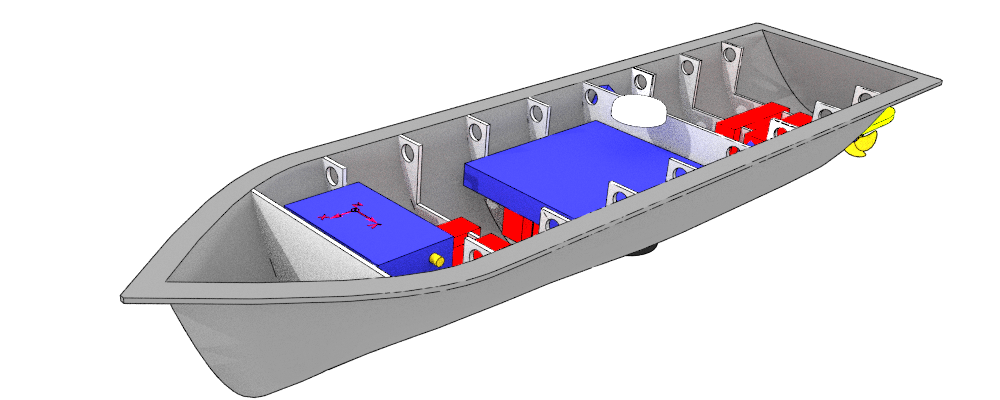
\includegraphics[width=13cm]{frontmatter/aauship}
\end{center}
\vfill
\begin{center}
	
\includegraphics[width=5cm]{frontmatter/AAU_LOGO_CMYK_UK}\\
	Department of Electronic Systems
\end{center}
\clearpage
% \restoregeometry

\frontmatter
\chapterstyle{nickoe}

%\layout
%  \includepdf{illustrations/cover}
%\cleardoublepage
%\input{formalities/titelbladdk}
\cleardoublepage
\thispagestyle{empty}
\newgeometry{right=2cm}
\noindent
\begin{minipage}[l]{0.50\textwidth}
	\centering
	
\includegraphics[width=3.35cm]{frontmatter/AAU_LAT_CIRCLE_blue_rgb}
\end{minipage}
\begin{minipage}[r]{0.50\textwidth}

\noindent
	\begin{tabular}{l}
		{\textsf{\small \textbf{Institute of Electronic Systems}}}\\
		{\textsf{\small \textbf{Control Engineering}}} \\
		{\textsf{\small Fredrik Bajers vej 7}} \\
		{\textsf{\small 9220 Aalborg \O st}} \\
		{\textsf{\small Phone 99 40 86 00}} \\
		{\textsf{\small http://es.aau.dk}}
	\end{tabular}
\end{minipage}


%\fbox{
\begin{minipage}[c]{0.45\textwidth}
	\begin{description}[leftmargin=\parindent+0.5em,labelindent=\parindent]
	\item [\textbf{Title:}] \tightlist
	\item Formation Control of Autonomous Surface Vehicles for Surveying Purposes
	\end{description}

	\begin{description}
	\item [\textbf{Theme:}] \tightlist
	\item Master’s thesis
	\end{description}

	\begin{description}
	\item[Projectperiod:] \tightlist
	\item 2014
	\end{description}
	%  \hspace{4cm}
	\begin{description}
	\item[Projectgroup:] \tightlist
	\item 1034
	%  \hspace{4cm}
	\end{description}

	\begin{description}
	\item[Participants:] \tightlist
	\item Nick \O stergaard 
	\item Jeppe Dam
	\end{description} 

	\begin{description}
	\item[Supervisor:] \tightlist
	\item Jesper Abildgaard Larsen
	\end{description}

	\begin{description}
	\item[Number of printed copies:] 2
	\item[Number of pages:] \arabic{lastsheet} 
	\item[Appendices:] ??\todo{update} + website
		\footnote{Website with additional material, \url{http://kom.aau.dk/group/14gr1034/attached}}
	\item[Finished on:] \today
	\end{description}
\end{minipage}
\hfill
\begin{minipage}[r]{0.50\textwidth}
	{\textbf{Synopsis:}} \\
	\fbox{\parbox[c]{\textwidth-0.5em}{
	\bigskip
	{\vfill{\small \lipsum[1]

	\bigskip}}
    }}
\end{minipage}
%}
\vfill
\begin{center}
	
\includegraphics[width=1.35cm]{frontmatter/ca-logo.pdf}
\end{center}
\restoregeometry

%Rapporten skal afleveres til følgende:
%1 stk. til hovedvejlederen (afleveres til studiesekretæren)
%1 stk. til censor (afleveres til studiesekretæren)
%1 stk. til hver studerende i gruppen

\chapter{Preface}
\todo[inline]{This has to be written some time in the future, describe what this doc is.}

\subsubsection*{Thanks to}
\todo[inline]{Say thanks to someone, Aalborg Havn if they are helpfull? Karl D. has been glad to answer ROS related questions.}


\begin{center}
  \begin{minipage}[t]{0.47\textwidth}
    \centering \vspace{1.5cm} \hrule \vspace{1mm} Nick \O stergaard
  \end{minipage}
  \hfill
  \begin{minipage}[t]{0.47\textwidth}
    \centering \vspace{1.5cm} \hrule \vspace{1mm} Jeppe Dam
  \end{minipage}
\end{center}


\newpage
\section*{Reading guide}
The following report is divided into parts, related to different phases of the project. The parts are divided into chapters, the chapters describe different aspects of the project. The chapters are subdivided a number of times to further split up the content into specific topics. The report is ended with an appendix part, that contains all the material that is relevant to the project, but not necessarily interesting to the reader, such as measurement journals and transcripts of meetings.

\begin{description}
\item[Citations] in the report is done according to the Harvard method, the list of references can be found \vpageref{ch:litt}. The elements on the list of references are sorted by author.
\item[Acronyms] are written to their full extend, the first time they are used, with the acronym in parentheses, thereafter only the acronym is used. The list of acronyms can be found \vpageref{ch:acronyms}.
\item[Notation] of vectors are written in bold font with lower case letters ($\vec{v}$), matrices are written in bold font with upper case letters ($\vec{M}$). Single variables and constants are typeset in normal math ($x$).
\item[Attached] to the report is a CD, which contains copies of web references and other digital files (source code, scripts and raw measurement data) that could be of interest to the reader. In some places in the report there will be a reference to the CD; this will look like this: \cd{/path-to-file}.
\end{description}


%%%%%%% Maybe we should have an overview of the system here
\cleardoublepage
\tableofcontents
\chapter{Acronyms}
\label{ch:acronyms}
\begin{acronym}[TDMA]
%\begin{acronym}[HBCI]
	\acro{AAU}{Aalborg University}
  \acro{ASV}{Autonomous Surface Vessel}
	\acro{ADC}{Analog to Digital Converter}
  \acro{AHRS}{Attitude and Heading Reference System}
  \acro{BODY}{The body frame}
  \acro{CFD}{Computational Fluid Dynamics}
  \acro{DOF}{Degrees-Of-Freedom}
  \acro{DP}{Dynamic Positioning}
  \acro{ECEF}{Earth-Centered Earth-Fixed} 
  \acro{ECI}{Earth-Centered Inertial}
  \acro{EKF}{Extended Kalman Filter}
  \acro{FRF}{Formation Reference Frame}
  \acro{FRP}{Formation Reference Point}
	\acro{GNC}{Guidance, Navigation and Control}
  \acro{GNSS}{Global Navigation Satellite System}
  \acro{GPS}{Global Positioning System}
  \acro{GRS}{Ground Segment}
  \acro{HLI}{High Level Interface}
  \acro{IMU}{Inertial Measurement Unit}
	\acro{IP}{Internet Protocol}
	\acro{IPv4}{Internet Protocol version 4}
	\acro{IPv6}{Internet Protocol version 6}
  \acro{KF}{Kalman Filter}
  \acro{LKF}{Linear Kalman Filter}
  \acro{LOS}{Line-Of-Sight}
  \acro{LLI}{Low Level Interface}
	\acro{LSB}{Least Significant Bit}
  \acro{LTI}{Linear Time Invariant}
  \acro{MARG}{Magnetic, Angular Rate, and Gravity}
  \acro{MMSE}{Minimum Mean Square Error}
  \acro{MUV}{Multiple Unmanned Vehicle}
  \acro{MPC}{Model Predictive Control}
  \acro{NED}{North-East-Down}
  \acro{OSM}{OpenStreetMap}
  \acro{PWM}{Pulse Width Modulation}
  \acro{ROS}{Robot Operating System}
  \acro{RTK}{Real Time Kinematic}
  \acro{SOG}{Speed Over Ground}
  \acro{SSS}{Single Screw Ship}
  \acro{SSM}{State Space Model}
  \acro{TSS}{Twin Screw Ship}
  \acro{UGAS}{Uniformly Globally Asymptotically Stable}
  \acro{UGES}{Uniformly Globally Exponentially Stable}
  \acro{UGS}{Uniformly Globally Stable}
  \acro{UKF}{Unscented Kalman Filter}
  \acro{WGS84}{World Geodetic System 1984}
\end{acronym}



\mainmatter
\descpart{Introduction}{In this part is the motivation for the project stated and the previous work within the subject will be summed up.}
\chapter{Introduction}
% \chapter{Introduction}
\head{In this chapter is the motivation for the project stated and the previous work within the subject will be summed up.}

\section{Motivation and the AAUSHIP Project}
The Port of Aalborg would like Aalborg University to help them to expand their options of improving the conditions of the Limfjord. One of their tasks is to map the seabed of the Limfjord to get bathymetry data. This will help them guide larger cargo ships to port while using the autonomous ships as guidance.

Another aspect from The Port of Aalborg is a task to escort larger ships with cargo into The Port of Aalborg. This is done by a pilot whom needs to sail out to incoming larger cargo ships and escort them safely into port. The pilot does this in a pilot boat which is controlled manually by the pilot. The Port of Aalborg would like this process to become autonomous such that an autonomous boat can sail to the cargo ship and to some extend take over the control and guide the cargo ship into port. The system to do this implies that The Port of Aalborg needs an autonomous ship which can perform this task.

The mapping itself can be done by one ship or by more. For the moment one of the ships from The Port of Aalborg, which is manned, and covers the mapping of the closer part of the Limfjord ($\approx$ 65 km). This is only done every third year, but mapping around Hals Barre (a sandbar \todo{slet efterfølgende kommentar igen engang}and not a beach bar) at the end of the Limfjord is a more critical place and is mapped every third month.

If The Port of Aalborg had an autonomous ship fleet at their disposal, which could sail out and do the mapping autonomously, they would get updated bathymetry maps with a higher update frequency than they have currently \citep{portofaalborg}. This will result in a digitalizing of the seabed, a digital map, which has different implementation options by The Port of Aalborg.

This thesis will utilise formation control and extensions to manoeuvre agents through a specified area for surveying purposes. The aspect of formation control is chosen due to the rather large areas that The Port of Aalborg needs so cover. When applying formation control it is assumed to be faster to cover a larger area than if one single boat needed to scan the area. The formation that are to be chosen depends on the specific area of interest, which could e.g. be inside the harbour or around the pillars of the bridge. Chapter~\vref{ch:formcontrol} will introduce what kind and scopes of formation control that exists today. These theories makes the basis for the formation control within the scope of this project.

As a future scope this can be used when making a model of the seabed of how this will get sanded. This model can tell The Port of Aalborg when to go clean the seabed. The AAUSHIP project can be used to verify this model, such that The Port of Aalborg do not have to go out with equipment to solve the sanding without the need of it.

\section{The Mission}
\label{sc:mission}
Within the scope of this project the robots will be unmanned ships,
\ac{ASV}. The ship's main purpose will be to map the seabed by using
sonars to obtain bathymetry data. When one ship need to do this alone, and due to the range of
the sonar, the time spend could be improved by using multiple ships. The sonar scanning would
be done as seen on figure~\vref{fig:concept-art}.

\begin{figure}[htbp]
	\centering
	\subfloat[One ship\label{fig:concept-art1}]{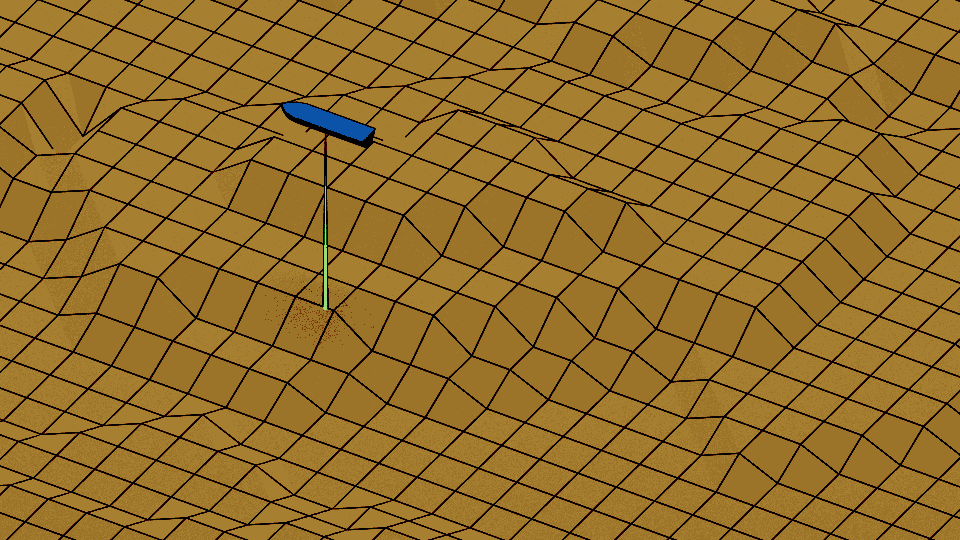
\includegraphics[width=0.48\textwidth]{fig/conseptart-single}}
	\ % One forced space to seperate figures
	\subfloat[Thee ships\label{fig:concept-art3}]{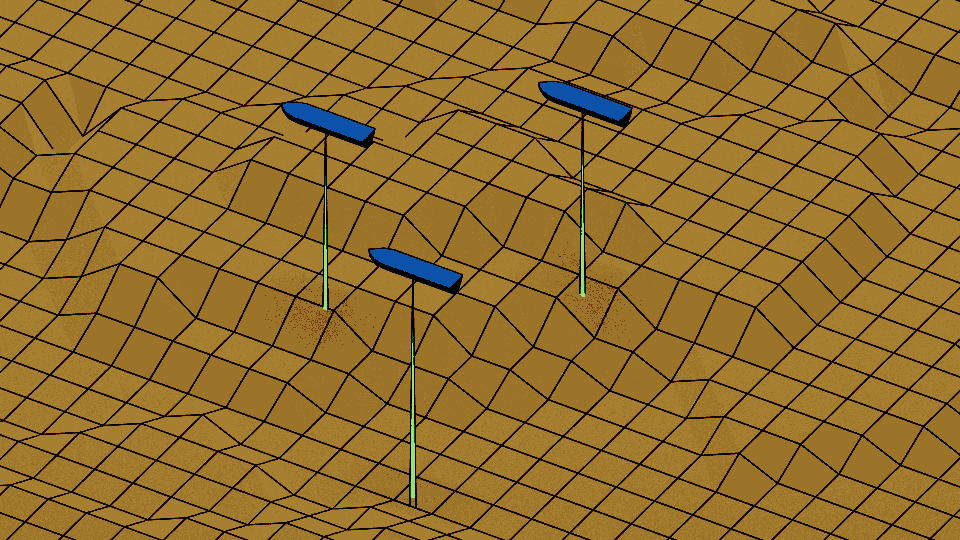
\includegraphics[width=0.48\textwidth]{fig/conseptart-formation}}
	\caption{Comparison of two ways to cover an area with a lawn mower
	pattern.}
	\label{fig:concept-art}
\end{figure}

When only one ship (figure~\vref{fig:concept-art1}) need to map a complete seabed this process could
take up much time dependent on the area that need to be covered. The
time spend could be improved to make this mapping more efficient. One
way of optimizing the time used is to add more ships (figure~\vref{fig:concept-art3}) to help map the
seabed. To make the process of this as optimal as possible it could be
of benefit to implement formation control in the specific assignment.

I cooperation with the port of Aalborg, a use case is presented, where we can perform tests of the platform, and use those to compare the performance of our system to their system.
\begin{figure}[htbp]
	\centering
	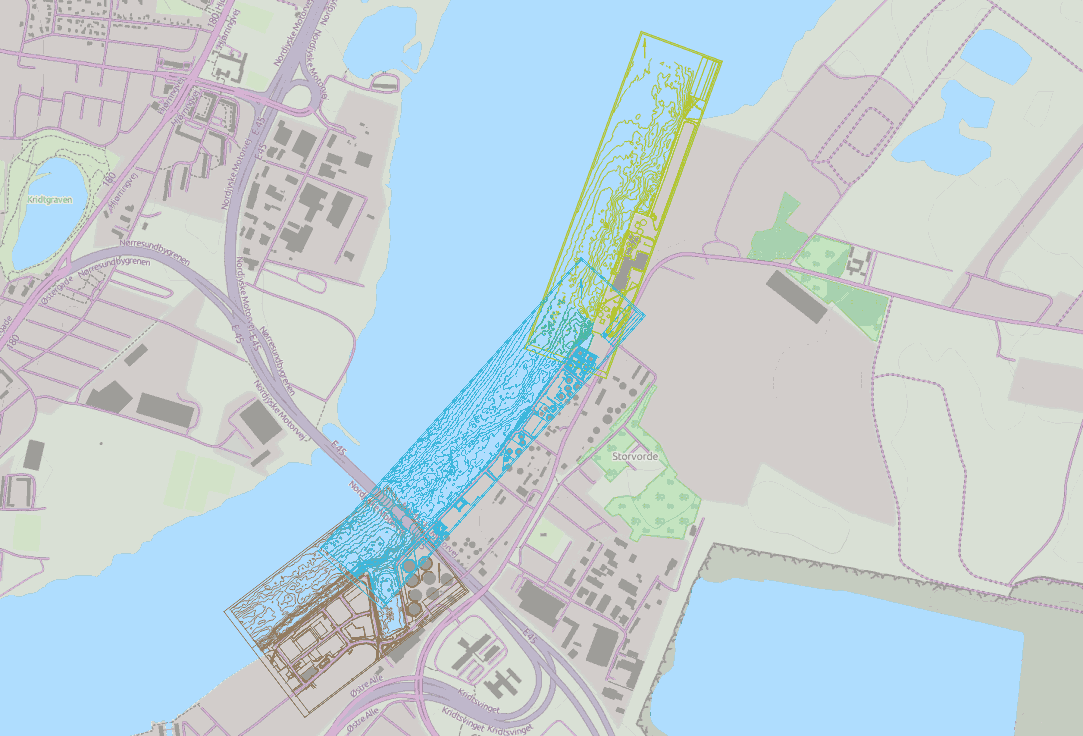
\includegraphics[width=\textwidth]{fig/use-case-data}
	\caption{Area of the harbour at Aalborg Portland provided as sample
	data from Aalborg Havn. Background map data CC BY-SA OpenStreetMap.}
	\label{fig:diffforms}
\end{figure}

When performing this kind of surveying with multiple ships, it is important to take note of the kind of sensor it uses and the coverage that it provides. Initially the port of Aalborg used single beam echo sounders, but have in recent years turned over to multibeam sonars for their survey boat, which has improved their resolution and time for a survey. But they still wishes to improve the survey update rate, by e.g. using fairly low cost autonomous ships to get better indication of the seabed to identify if an expensive thorough survey is needed. An image of the survey vessel they use now used can be seen on figure \ref{fig:alba}. As it can be seen, this survey vessel is relatively large, being over 20 metres long. To comparison is the AAUSHIP only 1.1 metres long. For surveying in smaller areas, like inside the harbour area, Aalborg Havn uses a smaller scale vessel which is 12 metres long. This vessel is only used at the smaller areas thus not the one being used out in the Limfjord close to Aalborg.
\begin{figure}
	\centering
	\includesvg{alba}
	\caption{The survey vessel used by Aalborg Havn named Alba.}
	\label{fig:alba}
\end{figure}



%This could be done in several ways, but is mostly thought of in a
%rigid formation, such that the formation maps the same area of the
%seabed the whole time. The idea can be seen on
%figure~\vref{fig:concept-art}.

\chapter{General formation control}
\head{This section will give a short introduction to formation control in general, by discussing existing formation control paradigms and relating them to the motivation of the AAUSHIP as a survey platform consept.}

%\head{Formation control in general is concerned with simultaneous control of dynamic systems. These systems is often referred to as agents where the objective of these is to maintain a static reference to a specified object. This object could be another agent witch then would be referred to as the leader. The other agents objective will then be to stay in the relative position to the leader within a static formation.}

The theory of formation control in general is widely applied. It is usually applied in assignments regarding control of robots which needs to be placed relative to each other. Depending on the given task of the robots, and which type of robots are in focus, the formation can be utilized in different ways \cite{muv-survey1}.

The robots can also be of various types: Driving vehicles, helicopters, aeroplanes, ships etc. which can be both manned and unmanned. The tasks that these robots needs to fulfill can vary greatly. Robots in groups in general have many purposes such as vacuum cleaning robots, who needs to clean a rather large area or flying swarm robots like quadcoptors who can make different kinds of assignments. When quadcoptors work as a combined group they could lift a certain amount of payload to achieve their goal as a group, or they could work individually in a network to do several smaller tasks. An example of how quadcoptors are working together can be examined at \citep{ethswarm}.

All the robots in the terminology of \cite{muv-survey} are called \textit{agents}. These agents move either individually or in formation. This formation can be rigid or be flexible. If the agents move in rigid formation they will keep their relative positions to each other and must not diverge from the formation. The formation could also be flexible which sometimes is preferable. If the distances between three agents on line are large, and an obstacle needs to be avoided, only one of the agents needs to move from this obstacle if the formation is flexible. This can be seen on figure~\vref{fig:form_avoid_right}.
\begin{figure}[htbp]
	\centering
	\includesvg[width=0.5\textwidth]{form_avoid_right}
	\caption{A flexible formation where the right agent avoids an obstacle.}
	\label{fig:form_avoid_right}
\end{figure}

\section{State of the art}
When looking into formation control many different types of control can be taken into control. The main types of formation control are separated into six different types, separated by \cite{muv-survey}, all under the main topic \textit{multiple vehicles coordination strategies}. The overview for this can be found in the survey paper \cite{muv-survey} who explains the six main types and a few alternations of these.

The theoretical views on control of \ac{MUV}'s behaviour are by \cite{muv-survey} divided into two classes; centralized and decentralized systems. If the system is centralized this means that all control of the formation is done on one agent, and the others receive information from the core agent. This form of system has the advantage that the core agent can optimize vehicle coordination, accommodate individual agent faults and monitor the accomplishment of the mission. The main disadvantage of this system is that if a fault should occur in the core agent this will affect and facilitate a failure of the whole system.

The opposite way of controlling the system would be in a decentralized way. This way of controlling the formation is inspired by the aggregation of birds and fish. This makes each agent able to communicate and share information in between. This means that each agent is given its own part of the complete objective and thus can only complete a part of it, like moving around an object to get to end point of a trajectory. The advantage is that faults in a single agent can be overlooked, thus more robust to faults, but can result in a less efficient objective outcome. A decentralized system may be more appropriate to scale up such that more agents can be included and the computational load can, in difference from the centralized system, be split up onto more agents.

The different types of coordination and control algorithms within centralized and decentralized systems include: \textit{behavioural-based}, \textit{virtual structure}, \textit{leader-follower}, \textit{graph-based} and \textit{potential field approaches}. Within these structures are the terms \textit{cooperation control} and \textit{formation control} used. Cooperative control focuses on the global task that the group of agents needs to fulfil, and the formation control is the actions performed by each agent which is shared with the other agents in the group. 
\begin{description}[style=nextline]
	\item [Virtual structure]
	In a virtual structure is the entire formation treated as a single entity. The behaviour coordination for a group of agents in a virtual structure is uncomplicated compared to the coordination of many agents, due to the making of one structure e.g. based on fixed distances between the agents. The disadvantage falls on the centralization due to the structure treated as a single entity. If a failure in this structure happen results in a failure in the entire structure.
	\item [Behaviour Based Methods]
	The behavioural based model employs several behaviours for each of the agents and the final control used to control the formation is derived from a weighting of the relative importance of each of the behaviours. This could for instance be navigational behaviours to enable a navigation to be the main goal while avoiding hazards and stay in formation. So if one agent needs to avoid a collision with an obstacle the rest of the group should not take this into account. Only that single ship needs to leave the formation and get back into formation again.
	\item [Leader-Follower Approaches]
	Applying leader-follower methods designates one agent as being the leader and the rest of the agents as followers. The following agents need to position themselves relative to the leader and maintain a desired relative position to the leader. This makes the simplicity to this method, but there is no feedback from the followers to the leader and thus makes that a disadvantage. Separation-separation and separation-bearing are two popular leader-follower formation controls, where the followers stay at specified separation and bearing from their designated leader. Within this method it is possible to split the group up into several smaller groups with their individual designated leader.
	\item [Potential Field Approach]
	Potential field approaches assigns potentials to agents to make a weighting between them. This weighting could for instance determine the relative distances between the agents. This is usually used when following a virtual leader, such that this process is only made relative to the agents within the structure. This method can make ensure a collision free formation when every agent has been assigned their potential weighting respectively. In this method obstacles can be included and have assigned potentials as well. This will become an avoidance radius from the specific object.
	\item [Graph Theory Approaches]
	When applying the graph theory method one assign every agent as a node and assign connections between the nodes. In graph theory this is denoted vertices and edges. The study with graph theory is mainly concentrated of the formation itself and related to changes within the structure. This can be related to the structure within a tree-structure which is used when assigning the formations in graph theory manor. This can be applied as communication analysis for the agents and consensus analysis can be of benefit. The edges between the nodes symbolizes the possible connections thus communication between them. The nodes that are connected are denoted as neighbours and are capable of communicating.
\end{description}

\subsection{Approaches on formation control}
When performing this kind of surveying with multiple ships, it is important to take note of the kind of sensor it uses and the coverage that it provides. Initially the port of Aalborg used single beam echo sounders, but have in recent years turned over to multibeam sonars for their survey boat, which has improved their resolution and time for a survey. But they still wishes to improve the update rate, by i.e. using fairly low cost autonomous ships.

\missingfigure{Picture of the port of Aalborg's survey boat.}

This does not have any relevant impact of how the mappings of the seabed would be due to the subsequent processing of the collected data from the maps.

Different formations of ships can be seen on figure~\vref{fig:diffforms}.
\begin{figure}[htbp]
	\centering
	\includesvg[width=0.5\textwidth]{diffforms}
	\caption{Different formations which the \ac{ASV}s can make.}
	\label{fig:diffforms}
\end{figure}

The formation of the ships may not need to be strictly rigid. Situations could appear where it would be of benefit to change the ship's formation. If the formation need to avoid an obstacle and one or more ships needs to go faster or slower, which leads to a change in the formation, it might be of benefit to regroup the formation which is faster to reach. An example can be seen on figure~\vref{fig:avoid}.

\begin{figure}[htbp]
	\centering
	\includesvg[width=0.5\textwidth]{form_avoid}
	\caption{A formation needs to go around an obstacle where the inner most ship chooses the shortest path and the formation regroups.}
	\label{fig:avoid}
\end{figure}

When doing the formation control it is important to figure out what one
want to achieve, and depending on the strategy and the formation type
some things are to be considered as requirements regarding how the
formation should work. In this discussion lawnmower patterns are considered. In this work thee ships are considered for simplicity, but it should be extensible to n-number of ships. The lawnmower patterns will suit well for the mapping of a seabed where one or more ships are to sail from shore to shore in a fjord.

\subsubsection{Initialisation}
When looking at the specific task several things needs to be taken into account. When starting the mission, the ships may start at positions that is not in the desired formation. It might be of importance that the ships are in
formation when they start tracking the desired track. Therefore some
attention must be given on how to make the ships initialize this
formation. This is referred to as the group coordination task. An approach is to make the ships sail individually to the
starting positions with a speed that makes them hit their respectively starting points at
the same time. If one reaches its start point much earlier
than the other it must stop, which is not wanted because it then can
drift out of position again. This basically means that there exists an initialization
phase and a tracking phase. The start heading should of
course align with the path at the start point such that the path following can begin with zero error. The ships could also target their group formation before starting at time zero at the path. This will eventually make the initialization take longer time but ensure that the ships have made the group coordination task and are ready to start at the path.

Another issue to be considered is to ensure that no ship at
any point in time reaches a minimum speed that is necessary for the
ship to not drift out of formation. This could be a problem in corners
of the formation if a stiff construction, where the inner most ship
has to move slower, to accommodate the shorter distance on an inner
circle arc.

Faults like blackout on a ship could also be considered in the control
design. I.e. what happens with the formation when one ship faults in a
blackout. Should the rest of the formation stop, should the formation
still follow this drifting ship or should the mission simply terminate
when it is discovered that a ship has blackout. This is under the assumption that the formation is decentralized and every ship has its own control and is not controlled from a mother ship.

In the initialization phase it is also relevant to consider how the
ships should avoid each other if they are on the wrong side of each
other. If it is of benefit that a specific ship is at the most inner route, and is located at an outer position before the group coordination, this ship needs to cross the formation to get to the desired starting position. This initialization needs to be adjusted in the initialization phase to ensure that no ships collide.

\begin{figure}[htbp]
	\centering
	\includesvg[width=0.4\textwidth]{cornoring}
	\caption{Two ships initializing and following the path offset
		equally on each side, ships are constrained to sailing parallel
		and heading the same as path when projected onto the path. Blue
	dot is start of path. Fully drawn splines is initializing phase.}
	\label{fig:cornoring}
\end{figure}

On figure~\vref{fig:cornoring} is a simple path following performed
with two ships in a stiff formation with an equal distance from the
path. It illustrates four steps. In step \#0 the ships initializes a
random position near the start of the path being the group coordination task. At \#1 it is tracking the
path in formation, whilst still in formation. This is referred to as a formation coordination task. At \#2, the green
(right) ship is in a tight inner curve where it is important to
consider design of the path such that the capabilities of the ship is not
exceeded to stay in formation. At \#3 it is back to straight line path
following in formation. \citep{thorvaldsen}.

\begin{figure}[htbp]
	\centering
	\includesvg[width=0.6\textwidth]{form_rigid_90}
	\caption{Three ships in formation needs to make a 90\textdegree turn and stays in their relative positions and keeps the rigid formation.}
	\label{fig:form_rigid_90}
\end{figure}

When the ships needs to make a turn about something they can do it in many ways. On figure~\vref{fig:form_rigid_90} the ships keep their formation whilst turning about the object. When they reach the other side and have finished their turn, the ships have kept formation but the outer most ship has now become the inner most ship. The reason to turn like this could be that the inner most ship, the yellow ship, cannot turn as sharp as demanded to stay the inner most ship. Therefore, instead of turning the formation, they stay geometrically rigid.

\begin{figure}[htbp]
	\centering
	\includesvg[width=0.6\textwidth]{form_change_90}
	\caption{Three ships in formation needs to make a 90\textdegree turn and changes their relative positions.}
	\label{fig:form_change_90}
\end{figure}

As seen on figure~\vref{fig:form_rigid_90} the ships could have benefit of turning like this. This way of turning could cause trouble in the top of the turn, where the ships eventually will collide due to errors and the relative close distance to each other. This way could be altered a little such that the ships will turn like on figure~\vref{fig:form_change_90}. There the ships adjust their position and velocities to ensure that they will not collide, but they will therefore leave their formation shortly to return back into position again.

\subsubsection{Degree of Actuation}
The degree of actuation is a matter that sets some limitations on how
the path following can be made, and thus the methods available to
control the ships.

AAUSHIP is a ship, which means that is is not fully actuated in the
whole 3D space, but this is not needed since it is moving on a
surface. To be fully actuated it must be able to have controls for
surge, sway and yaw.

There are different ways of controlling, and a few could be:
\begin{description}[style=nextline]
	\item [Three or more controls]
	When having three or more control parameters it is said that the vessel is fully actuated. This way of controlling is usually used in low-speed manoeuvring and stationkeeping mostly by offshore \ac{DP} vessels.
	\item [Two controls and Trajectory-Tracking control]
	Trajectory-Tracking is done in a three \ac{DOF} system, $e(t)\in\mathds{R}^2\text{X}S$. It is done with two control inputs, $u(t)\in\mathds{R}^2$. This means that the control problem is underactuated which cannot be solved by linear control theory. A vessel under these terms is able to manoeuvre along a path with constant sideslip angle using only surge and yaw. This is the classic approach for path following.
	\item [Two controls and Weather-Optimal heading]
	When taking the weather conditions, and in general the environmental disturbances, into account, it is done as a mean of all the disturbances. This is used to stabilize the vessel regarding the position. It is done by making the heading depend of the change in the mean of the environmental disturbances.
	\item [Two controls and Path-Following control]
	The standard way by having two controls, being surge and yaw, and achieving path-following, is to define a 2-D workspace. This workspace is placed along the trajectory with along-track and cross-track vectors that are to represent the error to minimize. This is usually done by applying the \ac{LOS} path following controller that makes use of surge and yaw to accomplish the path following. This implies that a six \ac{DOF} system model needs to be internally stable such that only the two control inputs are used.
	\item [One control]
	This is only done with systems with three \ac{DOF} and is normally only used to stationkeeping.
\end{description}
\citep{fossen}

\subsection{Delimitations}
Within the scope of the AAUSHIP project will the focus be to apply and extend a leader-follower approach at the ships. This will include several tasks. The two main tasks will be to make a group coordination task and a formation coordination task. The group coordination task will be, as described earlier, an objective to get the ships into the desired formation before or exactly at the starting point of the path following. The formation coordination task will be to make a leader, virtual or not, follow a predetermined path set by waypoints. The path should be generated from waypoints placed on a map due to that the ship needs to travel over larger distances. This will make a waypoint based follower where the path will be generated between the placed waypoints.

The placement of the waypoints will be placed such that the ships need to surge along a lawnmower pattern, where the turns have a lower requirement of turn radius dependent on the surge velocity of the most inner ship. This is due to the drift if the inner ship looses too much velocity.

When applying the leader-follower approach it needs to be determined how the formation precisely should be set up. In this project is only one leader considered at a time. The rest of the ships will act as followers to the leader. The idea can be seen on figure~\vref{fig:l_f} where only one leader is represented with a single or more followers.
\begin{figure}[htbp]
	\centering
	\includesvg[width=0.6\textwidth]{lead_follow}
	\caption{A leader is always assigned and potential followers are following.}
	\label{fig:l_f}
\end{figure}
When the followers are in formation with the leader is only the leader who is following a specified trajectory. The other ships, the followers, only keeps their position relative to the leader. This makes the predetermined formation moving along the path relative to how the leader is following the path. The leader is autonomous as well as the followers, but the path following is only done at the leader and the followers maintains their relative positions to the leader.

If the leader diverges from the path, drifting to the left, this will result in the whole formation drifting to the left. This problem can be dealt with in different ways, e.g. the control could react fast enough to make the formation get back on track within a specified time, or some fault tolerance could be done from the whole system. If the leader diverges from the path it could make the formation stay at their respective headings within a time slot before actuating towards the leader.

The formation needs to take into account if it is of benefit to change leader. If some kind of obstacle makes the formation turn about it, it might come to benefit to change the leader which needs to be done on the fly. This entails a change in the group coordination and the ships needs to set their relative position and heading from another ship.

The configuration of the formation will be set up, as a start, with one leader and a single follower. The follower will be offset from the leader with a distance of five metres. This can be seen on figure~\vref{fig:l_f1}.
\begin{figure}[htbp]
	\centering
	\includesvg[width=0.4\textwidth]{lead_follow1}
	\caption{The leader with a follower offset by 5 metres radius.}
	\label{fig:l_f1}
\end{figure}
This will be a rigid formation that the ships needs to keep at all times. The change of leader will eventually be taken into account when the ships needs to turn. If the formation needs to turn clockwise about it might be of benefit to change the leader. 

The location to test and implementation the AAUSHIPs will be in the Limfjord. The optimum will be to make the formation go across the Limfjord and back in lawnmower pattern and make measurements of the seabed. Due to the location where it is presumed to have enough space, the formation is not of bigger importance to the mapping. The only important thing to include regarding the formation is that the ships needs to be able to turn around without loosing so much velocity such that they start drifting and offset the formation.


% \descpart{Preliminary analysis}{%
% This is da stuff that is roolin'.}

\descpart{Control Design}{}
\chapter{\acs{ROS} design}
\head{This chapter describes the details of the implementation level,
which is done on a \acl{ROS} platform. This should provide all the
information needed to complete the implementation.}

It was decided to use \ac{ROS} in the implementation, It is used as an
other abstraction layer on top of the \ac{LLI}. In turn making AAUSHIP
modular and make it easy for others to write parts of the control
system without reimplementing basic components. This in turn makes it
an extensible platform, that should be easy to extend. \ac{ROS} is a
project available at \url{http://ros.org}, which describes itself in
short as following:

\begin{quote}
\textit{\noindent
	ROS (Robot Operating System) provides libraries and
	tools to help software developers create robot applications. It
	provides hardware abstraction, device drivers, libraries,
	visualizers, message-passing, package management, and more. ROS is
	licensed under an open source, BSD license.
}
		
	\hfill ROS.org
\end{quote}

\section{\acs{ROS} terminology}
To start working with \ac{ROS} it is important to use the terminology
used by \ac{ROS} to avoid confusion. Therefore these  will be stated
in this section.  The idea of \ac{ROS} is to make it easy to build a
system modularly, and this is achieved byt using almost
``self-contained'' code segments called \textit{nodes}, which is
application parts that is run as its own process. A node should be
designed to execute limited tasks such as image processing or similar
atomic processes. These nodes can then communicate with other nodes by
the means of two main communication forms called \textit{topics} and
\textit{services}.

\begin{description}
\item[The topic] is an asynchronous connection, that can \textit{publish}
from many nodes and be \textit{subscribed} by many nodes. This means
that it is a multicast form for providing data.
\item[The service] is a synchronous connection that is used between one node
to another node. This is only unicast.
\end{description}

An illustration of multiple nodes connected via topics and a service
is on figure~\vref{fig:ros-node-simple-concept}. This concept can also
be used across multiple machines. This is illustrated in
figure~\vref{fig:ros-node-master-concept}. On this a new type of unique
node is introduced, this is the \ac{ROS} master. This is a required
component for a ROS system to run. The masters only purpose is to make
the nodes connect together via the topics or services. There can only
be one master per \ac{ROS} system. This also enables multiple machines
to share topics, by connecting the master that runs on one machine. In
short the masters sole purpose is to make these connections. It is
illustrated by the dashed arrows. Each node says that it want to i.e.
publish or subscribe to a certain topic. To connect a node from one
machine to another, the environment variable \texttt{ROS\_MASTER\_URI}
has to be set to the host with the master running, and the
\texttt{/etc/hosts} file has to be set on all machines with the other
machines hostnames.

\begin{figure}[htbp]
	\centering
	\includesvg{ros_node_simple_concept}
	\caption{Basic principle of the node abstraction illustrating a
	service and two topics. The topology chosen here is only to illustrate
	the possibilities.}
	\label{fig:ros-node-simple-concept}
\end{figure}

When that is said, that is not the whole picture of the topology. In a
need to make this flexible \ac{ROS} has made it such that the nodes
can be started and stopped kind of ``runtime''. That is such that it is
possible to have different configurations of nodes to run in different
scenarios, i.e. in development with debugging nodes and virtual sensor
nodes versus in the real mission where no debugging nodes is used and
real sensor nodes that use real sensor data is used.

\begin{figure}[htbp]
	\centering
	\includesvg{ros_node_master_concept}
	\caption{Concept showing the ROS master together with the nodes,
	also illustrating the masters role with multiple machines. Dashed
	lines hows that the node will either subscribe or publish to the
	topic. This only happens initially when connecting to a topic. Gray
	area is two physical separate but networked machines.}
	\label{fig:ros-node-master-concept}
\end{figure}

\section{ROS on AAUSHIP}
\begin{figure}[htbp]
	\centering
	\includesvg{ros_aauship_teleop}
	\caption{ROS configuration on AAUSHIP for manual tele operation.}
	\label{fig:ros-aauship-teleop}
\end{figure}


\chapter{Modelling}
\head{This chapter describes the modelling of AAUSHIP. This is
necessary to be able to use model based control algorithms and
estimators.}

\section{Hydrodynamic Modelling}
Hydrodynamic added mass is defined as the mass added to a system due to an accelerating or decelerating body that needs to move a volume of the surrounding fluid as it moves through it. To this is said that the object and fluid is not able to occupy the same physical space simultaneously.
\begin{align}
M_A \dot \nu_r + C_A(\nu_r)\nu_r + D(\nu_r)\nu_r + g(\eta_r) = \tau
\label{eq:hydmodel}
\end{align}
where
\begin{align}
&M_A \text{ is the added mass matrix from the system}\nonumber\\
&C_A \text{ is the added mass matrix due to the Coriolis force}\nonumber\\
&D(\nu) \text{ is both the potential and viscous damping matrices}\nonumber\\
&g(\eta) \text{ is the restoring forces, which is dependent on the position of the vessel}\nonumber\\
&\tau \text{ is control and propulsion forces}\nonumber\\
&\nu \text{ is the velocities of the vessel in all directions and moments}
\end{align}

\section{Rigid Body Modelling}
The rigid body is used to model the physics of the vessel. It is an idealisation of the solid body from where the physical motions of the vessel are to be derived. Translational motion and rotational motion be derived by analysis of this, and by \citep{fossen} written in component form as:
\begin{align}
f^b_b &= [X,Y,Z]^T & &- \text{force through } o_b \text{ expressed in } \{b\}\\
m^b_b &= [K,M,N]^T & &- \text{moment about } o_b \text{ expressed in } \{b\}\\
v^b_{b/n} &= [u,v,w]^T & &- \text{linear velocity of } o_b \text{ relative } o_n \text{ expressed in } \{b\}\\
\omega^b_{b/n} &= [p,q,r]^T & &- \text{angular velocity of } {b} \text{ relative to } \{n\} \text{ expressed in } \{b\}\\
r^b_g &= [x_g,y_g,z_g]^T & &- \text{vector from } o_b \text{ to CG expressed in } \{b\}
\end{align}

The rigid body forces are written as:
\begin{align}
M_{RB} \dot \nu_r + C_{RB}(\nu_r)\nu_r = \tau_{RB}
\label{eq:rigidmodel}
\end{align}
where
\begin{align}
M_{RB} &\text{ is the system inertia matrix}\nonumber\\
C_{RB} &\text{ is coriolis-centriopedal matrix}\nonumber\\
\tau_{RB} &\text{ is a lumped force combined of } \tau_{\text{hyd}} + \tau_{\text{hs}} + \tau_{\text{wind}} + \tau_{\text{wave}}\nonumber
\end{align}
where in $\tau_{RB}$
\begin{align}
\qquad \tau_{\text{hyd}} &\text{ is the hydrodynamic force}\nonumber\\
\qquad \tau_{\text{hs}} &\text{ is the hydrostatic force}\nonumber\\
\qquad \tau_{\text{wind}} &\text{ is the wind force}\nonumber\\
\qquad \tau_{\text{wave}} &\text{ is the wave force}\nonumber
\end{align}

\section{Total Model of Vessel}
\begin{align}
\underbrace{M_{RB} \dot \nu_r + C_{RB}(\nu_r)\nu_r}_{\text{rigid-body forces}} + \underbrace{M_A \dot \nu_r + C_A(\nu_r)\nu_r + D(\nu_r)\nu_r + g(\eta_r)}_{\text{hydrodynamic forces}}  = \tau + \tau_{RB}
\label{eq:totmodel}
\end{align}
\todo{Argumenter via reference til f.eks. fossen at vi kan se bort fra
nogle led. Er det en valid antagelse?}
\citep{fossen} \todo{lav lidt mere præcise refs til fossen som står lige førnævnt} Since the vessel within this project is of smaller scale, the $M_A$, $C_A$ and $C_{RB}$ from \ref{eq:hydmodel} and \ref{eq:rigidmodel} are neglected. $M_A$ is the added mass and is as a start omitted due to the tests needs to be made as an object moving through the water with some drag. If the model needs to be further improved in the process this is a place to start modelling. The coefficients of $M_A$ are rather inconvenient to determine without advanced equipment like a towing tank, where constant velocity can be applied and measure drag and more in all directions and moments. $C_A$ and $C_{RB}$ represents forces due to a rotation of the body frame, \{$b$\}, about the inertial frame, the NED frame. These are omitted as well due to the small vessel where the body frame is placed in a predefined local frame which acts as the NED frame. This reduces equation \ref{eq:totmodel} down to the following:
\begin{align}
M_{RB} \dot \nu_r + D(\nu_r)\nu_r + g(\eta_r) = \tau_{RB} + \tau
\label{eq:reducedmodel}
\end{align}
The damping matrix which contains the coefficients of the drag is denoted the hydrodynamic damping matrix. This consists both of $D$ which is the linear damping matrix due to potential damping and possible skin friction with the water and $D_n(\nu_r)$ which is the nonlinear damping matrix due to quadratic damping and higher order terms. This can be expressed as $D(\nu_r) = D + D_n(\nu_r)$. This will, as a start, be modelled as the linear part, being potential and viscous damping. At higher velocities will the nonlinear part become more dominant due to the quadratic terms of the velocity, thus is mostly used with faster vessels. The linear damping matrix $D$ contributes more at lower speed manoeuvrings and stationkeeping. Therefore is the damping matrix $D$ used, and is expressed by ~\citep{fossen} for a 6 \ac{DOF} system to be:
\begin{align}
D =-
\begin{bmatrix}
X_u & 0 & 0 & 0 & 0 & 0\\
0 & Y_v & 0 & Y_p & 0 & Y_r\\
0 & 0 & Z_w & 0 & Z_q & 0\\
0 & K_v & 0 & K_p & 0 & K_r\\
0 & 0 & M_w & 0 & M_q & 0\\
0 & N_v & 0 & N_p & 0 & N_r
\end{bmatrix}
\label{eq:6dofd}
\end{align}

The rigid-body system matrix of the vessel is given for a 6 \ac{DOF} system by ~\citep{fossen} as:
\begin{align}
M_{RB} &=
\begin{bmatrix}
m\boldsymbol{I}_{3x3} & -m\boldsymbol{S}(r^b_g)\\
-m\boldsymbol{S}(r^b_g) & \boldsymbol{I}_b
\end{bmatrix}
\nonumber\\
&=
\begin{bmatrix}
m & 0 & 0 & 0 & mz_g & -my_g\\
0 & m & 0 & -mz_g & 0 & mx_g\\
0 & 0 & m & my_g & -mx_g & 0\\
0 & -mz_g & my_g & I_x & -I_{xy} & -I_{xz}\\
mz_g & 0 & -mx_g & -I_{yx} & I_y & -I_{yz}\\
-my_g & mx_g & 0 & -I_{zx} & -I_{zy} & I_z
\end{bmatrix}
\end{align}

The restoring forces acting on the vessel, while not in zero angle position in pitch and roll, is given by the coefficients of the $g$ matrix. The restoring forces acts on the vessel when it is perturbed away from the steady state angle in both pitch and roll. Then vessel will, due to Archimedes law, move back into steady state. The change in mass under waterline will rotate back to steady state and the change in angle will become zero. The coefficients in $g$ is the nonlinear terms contributing to the restoring force. Though it can be convenient to use the linear approximation, defined for a 6 \ac{DOF} system by \citep{fossen}, as:
\begin{align}
g(\eta) \approx G\eta
\end{align}
where $G$, for an asymmetric vessel, is defined as:
\begin{align}
G = -
\begin{bmatrix}
0 & 0 & 0 & 0 & 0 & 0\\
0 & 0 & 0 & 0 & 0 & 0\\
0 & 0 & -Z_z & 0 & -Z_\theta & 0\\
0 & 0 & 0 & K_\phi & 0 & 0\\
0 & 0 & -M_z & 0 & M_\theta & 0\\
0 & 0 & 0 & 0 & 0 & 0\\
\end{bmatrix}
\end{align}

This will be reduced to a 5 \ac{DOF} system due to the fact that the
vessels buoyancy cannot be controlled as such. The vessel will always
be on the water surface and this removes the degree of freedom which
is the heave, the change of $z$ position of the vessel. A 5 \ac{DOF}
system will be modelled as;
\begin{align}
M_{RB} =
\begin{bmatrix}
m & 0 & 0 & mz_g & -my_g\\
0 & m & -mz_g & 0 & mx_g\\
0 & -mz_g & I_x & -I_{xy} & -I_{xz}\\
mz_g & 0 & -I_{yx} & I_y & -I_{yz}\\
-my_g & mx_g & -I_{zx} & -I_{zy} & I_z
\end{bmatrix}
\end{align}
and
\begin{align}
D = -
\begin{bmatrix}
X_u & 0 & 0 & 0 & 0\\
0 & Y_v & Y_p & 0 & Y_r\\
0 & K_v & K_p & 0 & K_r\\
0 & 0 & 0 & M_q & 0\\
0 & N_v & N_p & 0 & N_r
\end{bmatrix}
\label{eq:damping-matrix}
\end{align}
and
\begin{align}
G = -
\begin{bmatrix}
0 & 0 & 0 & 0 & 0\\
0 & 0 & 0 & 0 & 0\\
0 & 0 & K_\phi & 0 & 0\\
0 & 0 & 0 & M_\theta & 0\\
0 & 0 & 0 & 0 & 0\\
\end{bmatrix}
\label{eq:restoreforce}
\end{align}
where the heave are neglected from the 6 \ac{DOF} system. In the principle could a 3 \ac{DOF} system be enough to make the control to the vessel and make it manoeuvre in the water, but as the scope is to exploit the sonar to map the seabed it would be beneficial to implement the roll and pitch as well and make the system as a 5 \ac{DOF}. The $G$ matrix has been reduced under the assumption that there exists yz symmetry, which is a good assumption based on the design of the vessel.

\section{Identification of Hydrodynamic Derivatives}
\label{sec:hydrocoeff}
The linear model \eqref{eq:reducedmodel1}, which is used to model AAUSHIP, consists of the mass matrix $M_{RB}$, the damping matrix $D$ and the restoring force matrix $G$. This makes the system as:
\begin{align}
M_{RB} \dot \nu_r + D\nu_r + G\eta = \tau_{RB} + \tau
\label{eq:reducedmodel1}
\end{align}
The coefficients of the model needs to be determined before the model can be simulated and implemented. These coefficients can be determined in multiple ways. Often ship design companies are able to use \ac{CFD} to determine the coefficients, or make use of a towing tank to determine the coefficients. These applications are often expensive and proprietary. So a third method to do this is to perform tests to do approximations of the coefficients. To do so some assumptions needs to be made. The model is defined as:
\begin{align}
M_{RB} \dot \nu_r + D\nu_r + G\eta = \tau_{hyd} + \tau_{hs} + \tau_{wind} + \tau_{wave} + \tau
\end{align}
Since the tests will be performed in still water some of the forces can be neglected. The $\tau$ is the only force to be taken into account to perform the tests. This is the input to the vessel and a delimitation can be performed to make the system as \ref{eq:testsystem}, which is assumed while tests are performed:
\begin{align}
M_{RB} \dot \nu_r + D\nu_r + G\eta = \tau
\label{eq:testsystem}
\end{align}
The system is modelled as a 5 \ac{DOF} system and the necessary coefficients are found in appendix \ref{app:damping}.

% While testing, as seen in appendix \ref{app:damping}, the vessel will in one test surge straight forward, in the next only perform sway and in the last only perform a rotation. This will, in the second test, make the terms regarding rotation be zero. Therefore it becomes possible to determine the remaining coefficients. This is also done in the last test while rotating. By making the vessel be in the same position, then any movement in x and y can be neglected. This makes it possible to determine the damping while rotating. After these three tests it is possible to determine the last cross terms from the system. The equations to determine will look like:
% \begin{align}
% m \ddot x - X_u \dot x = \tau\\
% m \ddot y - Y_v \dot y = \tau\\
% I_z\ddot \psi - N_r \dot \psi = \tau
% \end{align}
% After determine the damping coefficients $X_u$, $Y_v$ and $N_r$ it is possible to determine the last parameters from the original system from \ref{eq:syseq}, and can be seen here:
% \begin{align}
% m \ddot y + mx_g\ddot\psi - Y_v \dot y - Y_r \dot \psi = \tau\\
% mx_g \ddot y + I_z\ddot \psi - N_v \dot y - N_r \dot \psi = \tau
% \end{align}
% $Y_r$ and $N_v$ are the only unknowns and the rest to be determined. The performed tests to measure these coefficients can be found in appendix \ref{app:damping}.

The system ends up being:
\todo{konkluder hvordan systemet ser ud med de fundne variable}
\chapter{Different Control Strategies}

\head{"A control system, that forces the system output $y(t)$ to track a desired output $y_d(t)$ solves a trajectory tracking problem" \citep{fossen}}.

\todo{Should this be included under the selecteed formation control strageties?}

\section{Trajectory Tracking Control}
When applying control to a vessel that needs to track a specified trajectory, then the type control will be classified according to the number of available actuators.This is usually split between surge, sway and yaw, which corresponds to forward motion, sideslip and turning.

A time varying reference trajectory for a vessel to track will be given as:
\begin{align}
\eta_d=
\begin{bmatrix}
N_d(t)\\
E_d(t)\\
\psi_d(t)
\end{bmatrix}
\end{align}
To achieve tracking and convergence to such a trajectory is minimization of the error the main objective, $e(t):=\eta(t)-\eta_d(t)$. Or given by the previous notation:
\begin{align}
e(t):=
\begin{bmatrix}
N(t)-N_d(t)\\
E(t)-E_d(t)\\
\psi(t)-\psi_d(t)
\end{bmatrix}
\end{align}

When designing a motion control system with this type of objective it is important to distinguish between the following three important control objectives:
\begin{description}[style=nextline]
	\item [Setpoint regulation]
	This is the most basic way of regulating. In this method it is usually a human operator that controls the setpoint or reference to the vessel. The controller will then be a regulator that usually brings the error of the control signal and the real value to zero.
	\item [Path-following control]
	The path-following control makes the vessel follow a path independent of time with no temporal constraints. The method is usually used on underwater vessels or vessels in transit between continents.
	\item [Trajectory-tracking control]
	When applying trajectory-tracking control, position and velocity of vessels should track the position and velocity of some time varying path reference signal. The feedback is a trajectory tracking controller to make the vessel converge to the trajectory. This is used when having course changing manoeuvres and speed changing along the trajectory. This could for instance be a change of speed in a turn of the vessel.
\end{description}

\subsection{Manoeuvring the Vessel Using the LOS Method}
Path-following problems for vessels are often solved by implementing \ac{LOS} algorithms. Opposite to other position control algorithms, where the vessel may be driven both in longitudinal and transversal directions to converge to a path, the \ac{LOS} algorithm gives a more natural motion towards the desired path. This is done by giving a more natural reference to the heading of the vessel. One of the advantages of this is that it can be applied both to fully actuated and under actuated vessels.

Since it is only the leader, and not any of the followers, who need to follow a path, this is only applied on one vessel. This can also be extended to a leader in a virtual structure. To apply the \ac{LOS} algorithm a setup is needed. To get an overview of the functionality of the \ac{LOS} algorithm see figure~\vref{fig:allinallframes}.
\begin{figure}[htbp]
	\centering
	\includesvg[width=\textwidth]{allinallframes}
	\caption{A vessel placed beside the path and uses the \ac{LOS} algorithm to get back on track.}
	\label{fig:allinallframes}
\end{figure}
On the figure is a green vessel that needs to get onto the blue path. The red points at the path is way point positions $\theta$, $\textbf{p}_d(\theta)$. From this point a tangent to the path is made, which crosses the vessels heading and is along the path. The angle from north to the tangents slope (the path) is the \textit{desired heading}, $\psi_d$, for the vessel. This will make it converge to the reference path over time. $s$ along the tangent is the \textit{along track error}(tangential to path) and $e$ from the vessel to the path is the \textit{cross track error}(normal to path), which are two distances that needs to be minimized to make the vessel converge to the path. The along track error is not of great interest when applying a \textit{lookahead-based steering} where only the cross track error is of importance. The lookahead distance along the track is denoted $\Delta$ and is the distance from the normal at the path to the point of \ac{LOS} at the path.

\subsubsection{The \ac{LOS} Algorithm}
The vessel has a generalized position in the ${n}$-frame given as
\begin{align}
\eta = (\textbf{p},\psi)^\top\quad , \quad \textbf{p} = (x,y)^\top
\end{align}
with dynamics given by
\begin{align}
\dot{\eta} = \textbf{R}(\psi)\boldsymbol{\nu}
\end{align}
where $\boldsymbol{\nu} = (u,v,r)^\top$.\\
The path can be parametrized by a set of points with
\begin{align}
\mathcal{P} = {\textbf{x}}\in\mathds{R}^2 : \quad \exists \theta \in \mathds{R} \quad s.t. \quad \textbf{x} = \textbf{p}_d(\theta)
\end{align}
where $\textbf{p}_d(\theta) := (x_d(\theta),y_d(\theta))^\top$ is a smooth function. The path needs to be smooth such that the \ac{LOS} algorithm makes the vessel converge to the path. When applying the \ac{LOS} algorithm it makes the setup immune to sideslip error. This is due to the minimization of $e$ when the vessel approaches towards the path.

For a given value of $\theta$, being a specific point on the path, is the tangent to the path introduced with origin located in $\textbf{p}_d(\theta)$. The orientation of the reference frame, being the desired heading, is given by
\begin{align}
\psi_d(\theta) = \arctan2\left(\frac{y_d^\theta(\theta)}{x_d^\theta(\theta)}\right)
\end{align}
which then will be
\begin{align}
\psi_d = \arctan2\left(\frac{E}{N}\right)
\end{align}
The position of the vessel from the orthogonal position on the path is given in path-tangential coordinates according to
\begin{align}
\epsilon(\textbf{p},\theta) = (s(\textbf{p},\theta),e(\textbf{p},\theta))^\top
\end{align}
where $s(\textbf{p},\theta)$ is the along track error and $e(\textbf{p},\theta)$ is the cross track error. These are given on figure~\vref{fig:allinallframes}, and is the errors from the vessel to the desired point on the path. This position can also be expressed using the rotation of the $\epsilon$-vector by
\begin{align}
\epsilon(\textbf{p},\theta) = \textbf{R}_{2D}(\psi_d(\theta))^T(\textbf{p}-\textbf{p}_d(\theta))
\end{align}
where
\begin{align}
\textbf{R}_{2D}(\psi_d(\theta)) = 
\begin{bmatrix}
cos(\psi_d(\theta) & -sin(\psi_d(\theta)\\
sin(\psi_d(\theta) & cos(\psi_d(\theta)
\end{bmatrix}
\end{align}


\descpart{Simulation}{}

\cleardoublepage
\descpart{Appendix}{%
The appendix includes chapters which are important for the project, but not necessarily interesting to the reader of the report.}
\appendix
\includepdf[pages=-]{../manual/manual.pdf}


\backmatter
\bibliographystyle{apalike}
\bibliography{../manual/bib}
\label{ch:litt}

%\settocdepth{section}
\listoftodos
\end{document}

